\documentclass[aspectratio=169]{../latex_main/tntbeamer}  % you can pass all options of the beamer class, e.g., 'handout' or 'aspectratio=43'
\usepackage{dsfont}
\usepackage{bm}
\usepackage[english]{babel}
\usepackage[T1]{fontenc}
%\usepackage[utf8]{inputenc}
\usepackage{graphicx}
\graphicspath{ {./figures/} }
\usepackage{algorithm}
\usepackage[ruled,vlined,algo2e,linesnumbered]{algorithm2e}
\usepackage{hyperref}
\usepackage{booktabs}
\usepackage{mathtools}

\usepackage{amsmath,amssymb}

\DeclareMathOperator*{\argmax}{arg\,max}
\DeclareMathOperator*{\argmin}{arg\,min}

\usepackage{amsbsy}
\newcommand{\vect}[1]{\bm{#1}}
%\newcommand{\vect}[1]{\boldsymbol{#1}}

\usepackage{pgfplots}
\pgfplotsset{compat=1.16}
\usepackage{tikz}
\usetikzlibrary{trees} 
\usetikzlibrary{shapes.geometric}
\usetikzlibrary{positioning,shapes,shadows,arrows,calc,mindmap}
\usetikzlibrary{positioning,fadings,through}
\usetikzlibrary{decorations.pathreplacing}
\usetikzlibrary{intersections}
\pgfdeclarelayer{background}
\pgfdeclarelayer{foreground}
\pgfsetlayers{background,main,foreground}
\tikzstyle{activity}=[rectangle, draw=black, rounded corners, text centered, text width=8em]
\tikzstyle{data}=[rectangle, draw=black, text centered, text width=8em]
\tikzstyle{myarrow}=[->, thick, draw=black]

% Define the layers to draw the diagram
\pgfdeclarelayer{background}
\pgfdeclarelayer{foreground}
\pgfsetlayers{background,main,foreground}

% Requires XeLaTeX or LuaLaTeX
%\usepackage{unicode-math}

\usepackage{fontspec}
%\setsansfont{Arial}
\setsansfont{RotisSansSerifStd}[ 
Path=../latex_main/fonts/,
Extension = .otf,
UprightFont = *-Regular,  % or *-Light
BoldFont = *-ExtraBold,  % or *-Bold
ItalicFont = *-Italic
]
\setmonofont{Cascadia Mono}[
Scale=0.8
]

% scale factor adapted; mathrm font added (Benjamin Spitschan @TNT, 2021-06-01)
%\setmathfont[Scale=1.05]{Libertinus Math}
%\setmathrm[Scale=1.05]{Libertinus Math}

% other available math fonts are (not exhaustive)
% Latin Modern Math
% XITS Math
% Libertinus Math
% Asana Math
% Fira Math
% TeX Gyre Pagella Math
% TeX Gyre Bonum Math
% TeX Gyre Schola Math
% TeX Gyre Termes Math

% Literature References
\newcommand{\lit}[2]{\href{#2}{\footnotesize\color{black!60}[#1]}}

%%% Beamer Customization
%----------------------------------------------------------------------
% (Don't) Show sections in frame header. Options: 'sections', 'sections light', empty
\setbeamertemplate{headline}{empty}

% Add header logo for normal frames
\setheaderimage{
	% 
\includegraphics[height=\logoheight]{figures/TNT_darkv4.pdf}
	
\includegraphics[height=\logoheight]{../latex_main/figures/luh_logo_rgb_0_80_155.pdf}
	% 
\includegraphics[height=\logoheight]{figures/logo_tntluh.pdf}
}

% Header logo for title page
\settitleheaderimage{
	% 
\includegraphics[height=\logoheight]{figures/TNT_darkv4.pdf}
	
\includegraphics[height=\logoheight]{../latex_main/figures/luh_logo_rgb_0_80_155.pdf}
	% 
\includegraphics[height=\logoheight]{figures/logo_tntluh.pdf}
}

% Title page: tntdefault 
\setbeamertemplate{title page}[tntdefault]  % or luhstyle
% Add optional title image here
%\addtitlepageimagedefault{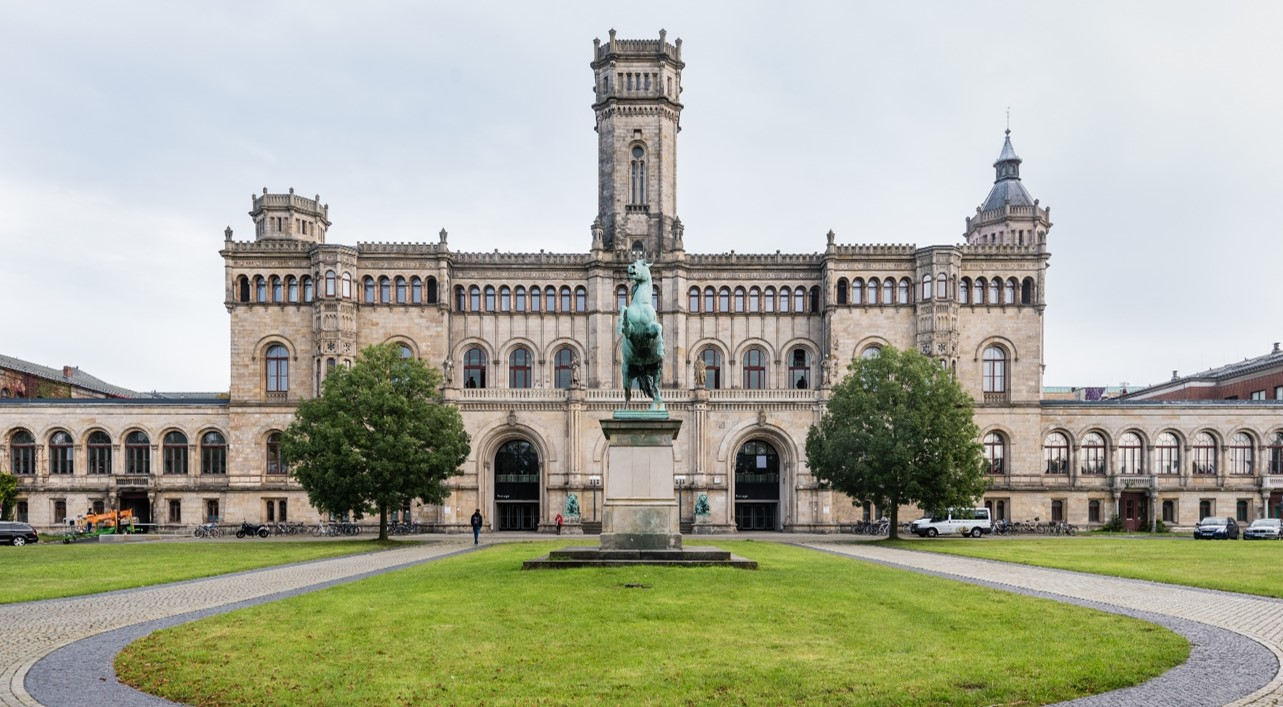
\includegraphics[width=0.65\textwidth]{figures/luh_default_presentation_title_image.jpg}}

% Title page: luhstyle
% \setbeamertemplate{title page}[luhstyle]
% % Add optional title image here
% \addtitlepageimage{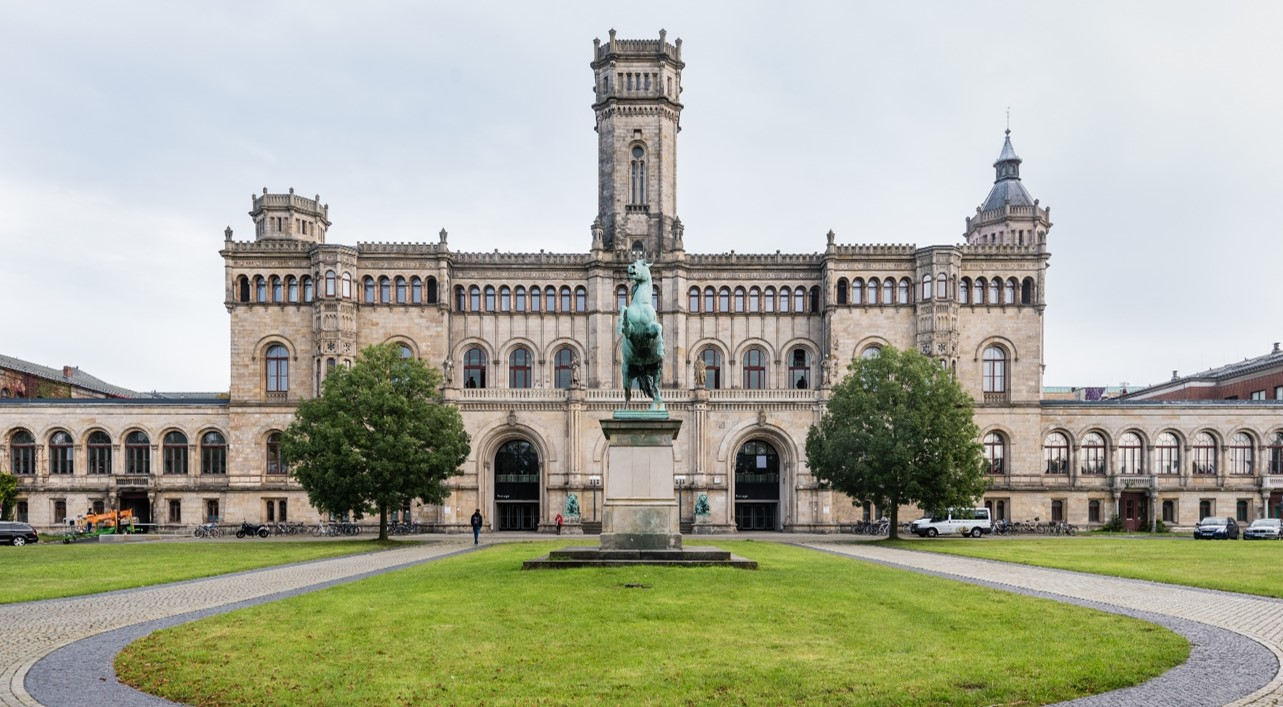
\includegraphics[width=0.75\textwidth]{figures/luh_default_presentation_title_image.jpg}}

\author[Abedjan \& Lindauer]{Ziawasch Abedjan \& Marius Lindauer\\[1em]
	
\includegraphics[height=\logoheight]{../latex_main/figures/luh_logo_rgb_0_80_155.pdf}\qquad
	
\includegraphics[height=\logoheight]{../latex_main/figures/DBIS_Kurzlogo.png}\qquad

\includegraphics[height=\logoheight]{../latex_main/figures/TNT_darkv4}\qquad

\includegraphics[height=\logoheight]{../latex_main/figures/L3S.jpg}	}
\date{Summer Term 2022; \hspace{0.5em} {
\includegraphics[height=1.5em]{../latex_main/figures/Cc-by-nc-sa_icon.svg.png}}; based on \href{https://ds100.org/fa21/}{[DS100]}
}


%%% Custom Packages
%----------------------------------------------------------------------
% Create dummy content
\usepackage{blindtext}

% Adds a frame with the current page layout. Just call \layout inside of a frame.
\usepackage{layout}


%%% Macros
%\renewcommand{\vec}[1]{\mathbf{#1}}
% \usepackage{bm}
%\let\vecb\bm

\title[Introduction]{DS: Estimation and Bias}
\subtitle{What is statistical bias?}

\graphicspath{ {./figure/} }
%\institute{}


\begin{document}
	
	\maketitle
	
	\begin{frame}[c]{Where we’re headed today}
	    What is statistical bias?\\
	    \hspace{4cm} The difference between your estimate and the truth.

	\end{frame}
	
		\begin{frame}{Interlude}
	    \begin{columns}
	        \begin{column}{.5\textwidth}
	     
	           \begin{figure}
	               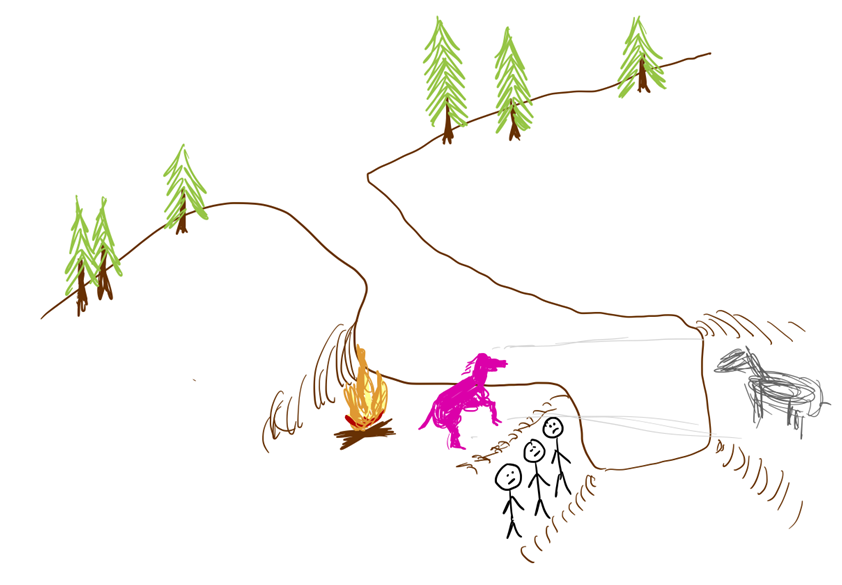
\includegraphics[scale=.55]{Bild24}
	           \end{figure}
	        \end{column}
	        
	        \begin{column}{.3\textwidth}
	            Plato’s Allegory of the Cave\\
	            \begin{itemize}
	                \item World of forms
	                \begin{itemize}
	                    \item Non-physical essence of all things
	                \end{itemize}
	                \item World of representation
	                \begin{itemize}
	                    \item The material world that we observe
	                \end{itemize}
	                \item Philosopher
	                \begin{itemize}
	                    \item Person who seeks knowledge of forms           
	                \end{itemize}
	            \end{itemize}
	        \end{column}
	        \end{columns}
	    
	\end{frame}
	
	
		\begin{frame}{Interlude}
	    \begin{columns}
	        \begin{column}{.5\textwidth}
	     
	           \begin{figure}
	               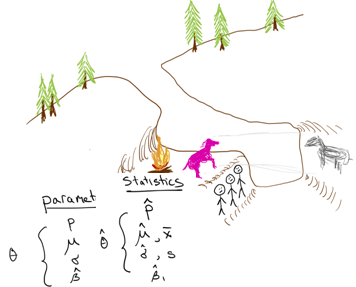
\includegraphics[scale=.75]{Bild23}
	           \end{figure}
	        \end{column}
	        
	        \begin{column}{.4\textwidth}
	            Metaphor of the Cave\\
	            \begin{itemize}
	                \item World of Parameters
	                \begin{itemize}
	                    \item Constants that define the structure of the world
	                \end{itemize}
	                \item World of Data / Statistics
	                \begin{itemize}
	                    \item Observable information generated by RVs and their parameters
	                    \item Statistic: numeric summary of data
	                \end{itemize}
	                \item Statistician
	                \begin{itemize}
	                    \item Person who uses statistics to learn about parameters
	                \end{itemize}
	            \end{itemize}
	        \end{column}
	        \end{columns}
	    
	\end{frame}
	
	
	\begin{frame}{What is a statistic?}
	    \begin{itemize}
	        \item A single piece of data
	        \item A numerical summary of a dataset
	        \begin{itemize}
	            \item function of realizations of RVs
	        \end{itemize}
	    \end{itemize}
	    \bigskip
	    \hspace{3cm}$\hat\theta = f(x_1,x_2,...,x_n)$\\
	    \hspace{3cm}What is an estimator?
        \begin{itemize}
            \item A statistic designed to estimate a parameter
        \end{itemize}
	\end{frame}
	
	
	\begin{frame}{Choosing a statistic/estimator}
	    \begin{columns}
	        \begin{column}{.4\textwidth}
	            Example 1: Squirrels\\
	           \begin{figure}
	               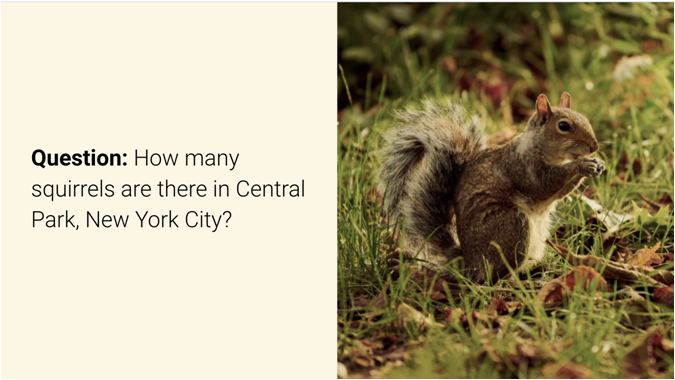
\includegraphics[scale=.6]{Bild25}
	               
	           \end{figure}
	        \end{column}
	        
	        \begin{column}{.5\textwidth}
	            \begin{figure}
                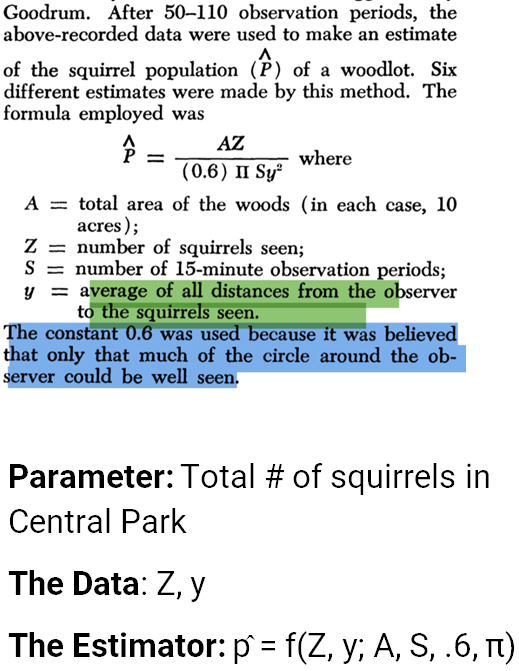
\includegraphics[scale=.33]{Bild26}
	                
	            \end{figure}
	        \end{column}
	        \end{columns}

	    
	\end{frame}
	
	
	\begin{frame}{Choosing a statistic/estimator}
	    \begin{columns}
	        \begin{column}{.4\textwidth}
	            Example 2: FDR vs. Landon\\
	            \bigskip
	            Question: what proportion of Americans will vote for FDR?\\
	           \begin{figure}
	               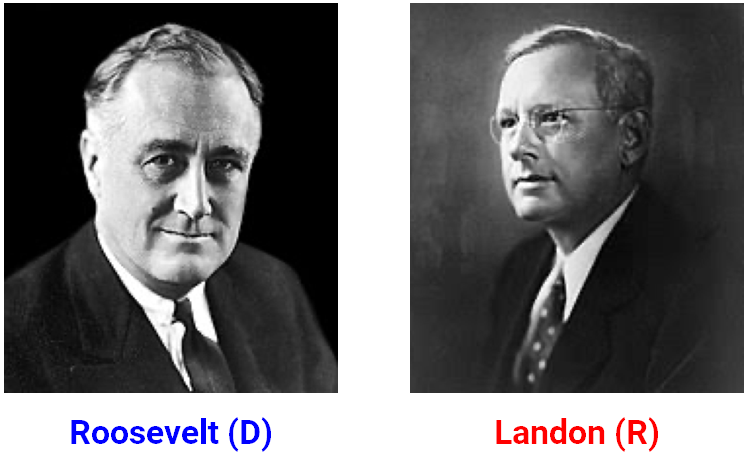
\includegraphics[scale=.3]{Bild27}
	           \end{figure}
	        \end{column}
	        
	        \begin{column}{.5\textwidth}
	            Parameter: The total proportion of votes for FDR, p\\
	            The Data: $X_1, X_2, ..., x_{10M}$\\
	            The Estimator:
                \begin{align*}
                    \hat{p} &= f(X_1, X_2,...,X_{10M};n)\\
                    &= (X_1, X_2,...,X_{10M})/n
                \end{align*}
	        \end{column}
	        \end{columns}

	    
	\end{frame}
	
	\begin{frame}[c]{What is statistical bias?}
	    \centering
	   The difference between your estimate and the truth.\\
        $\hat\theta - \theta$\\
        \bigskip
        Not quite...

	    
	\end{frame}
	
	
	\begin{frame}{Don’t forget about sampling variability}
	    \begin{columns}
	        \begin{column}{.4\textwidth}
	           Example: The total number of heads in a series of 5 coin flips: $Y = X_1 + X_2 + … + X_5$\\
	           \begin{figure}
	               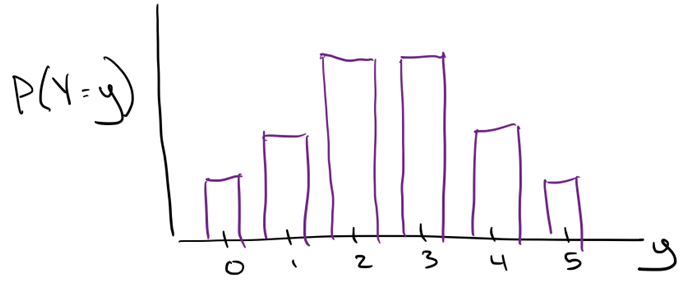
\includegraphics[scale=.5]{Bild28}
	           \end{figure}
	        \end{column}
	        
	        \begin{column}{.5\textwidth}
	           \begin{figure}
	               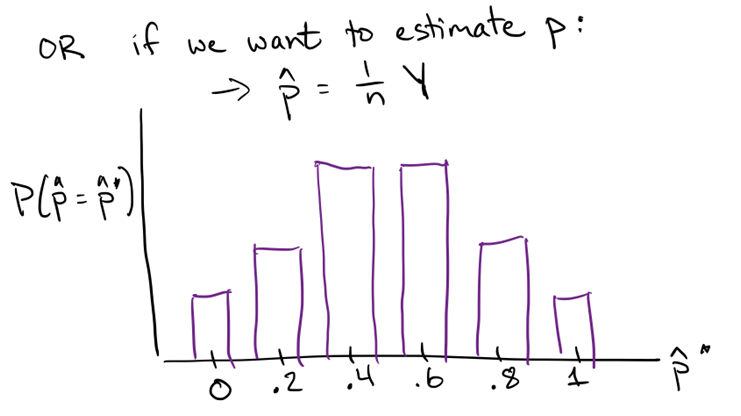
\includegraphics[scale=.5]{Bild29}
	           \end{figure}
	           \begin{itemize}
	               \item Y is an RV, therefore $\hat{p}$ is an RV
	               \item Since estimators are functions of RVs, they are RVs -> subject to sampling variability
	           \end{itemize}
	        \end{column}
	        \end{columns}

	    
	\end{frame}
	
	
	\begin{frame}{What is statistical bias?}
	    \begin{columns}
	        \begin{column}{.4\textwidth}
	           The difference between your estimate and the truth.
	           \begin{figure}
	               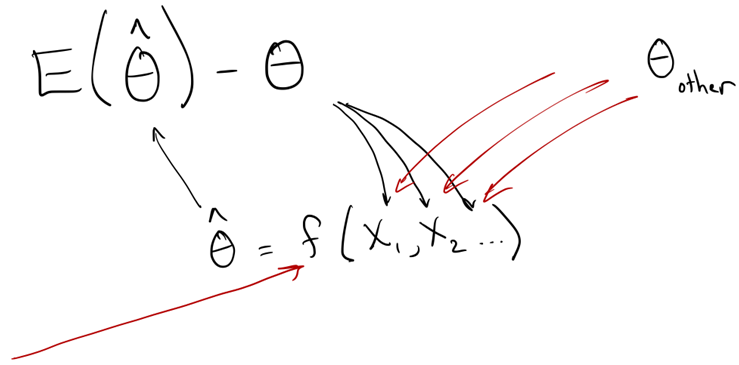
\includegraphics[scale=.31]{Bild30}
	           \end{figure}
	           Q: What if your estimator isn’t great?\\
	           A: Biased estimator\\
	           Ex. $ \hat{p_b}= Y_n / (n - 1)$

	        \end{column}
	        
	        \begin{column}{.4\textwidth}
	           \begin{figure}
	               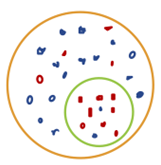
\includegraphics[scale=.5]{Bild31}
	           \end{figure}
	           Q: What if the data wasn’t generated by $\theta$ ?\\
	           \bigskip
	           A: It will not be representative of the population
                \begin{itemize}
                    \item Selection bias
                \end{itemize}

	        \end{column}
	        \end{columns}

	    
	\end{frame}
	
	
	\begin{frame}[c]{What’s Next?}
	    \begin{figure}
	        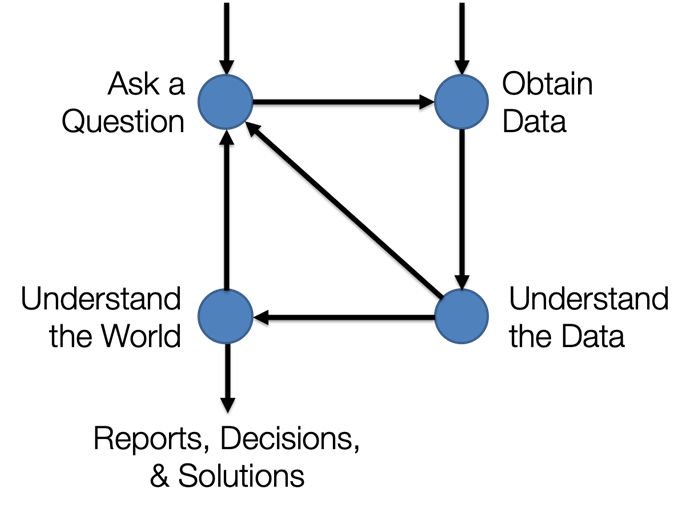
\includegraphics[scale=.5]{Bild1}
	    \end{figure}   
	\end{frame}
\end{document}